\begin{frame}[t]{Algoritmo Genético}
	
	O algoritmo genético é inspirado pelo evolucionismo, que se baseia em gerações de indivíduos, em que os mais aptos prevalecem e constroem a geração futura.
	
	\begin{figure}[h]
		\begin{center}
			\includegraphics[width=3cm]{./giraffe.jpg}   
		\end{center}
	\end{figure}
	
\end{frame}

\begin{frame}[t]{Algoritmo Genético}
	
	O primeiro passo para a construção do algoritmo genético é a criação de uma \textbf{primeira geração}, feita aleatoriamente, com quantidade de indivíduos e limites definidos.
	
		\begin{center}
			\animategraphics[autoplay,loop,width=5cm]{1}{frame_}{1}{5}
		\end{center}
	
\end{frame}
	
\begin{frame}[t]{Algoritmo Genético}
	O segundo passo é criar a \textbf{população intermediária}. O método escolhido para tal foi o canônico, com aptidão definida como 
	
	\begin{equation*}
		\phi_i = \dfrac{\bar{f}}{f_i}
	\end{equation*}
	
	Sendo
	\begin{itemize}
		\item $ \phi_i $ a aptidão do indivíduo $ i $.
		\item $ f_i $ a função objetivo avaliada no ponto do indivíduo $ i $.
		\item $ \bar{f} $ a média do valor da função para toda a população.
	\end{itemize} 
	
\end{frame}

\begin{frame}[t]{Algoritmo Genético}
	
	O terceiro passo é a recombinação, processo necessário para construir a \textbf{segunda geração}. O tipo de recombinação escolhido foi a média de três pais, para acelerar a convergência.
	
	\begin{figure}[h]
		\begin{center}
		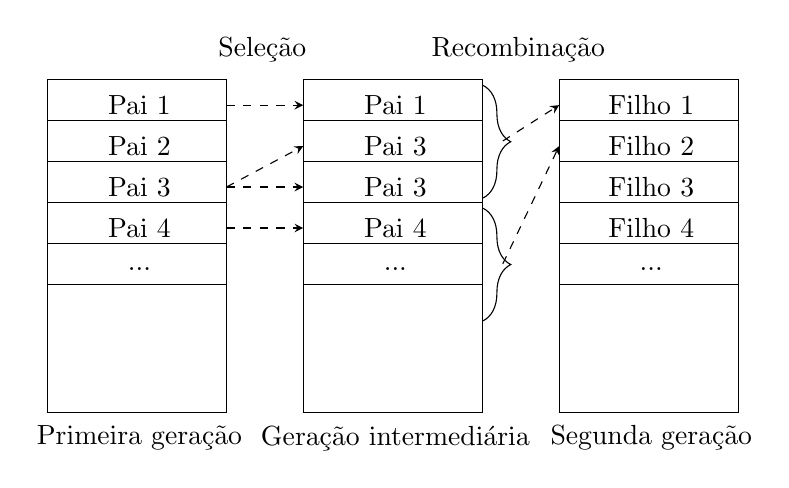
\begin{tikzpicture}[scale = 0.65]
		
		
		\draw  (-5.0,4.0) rectangle (-1.5,-2.5);
		\draw  (0.0,4.0) rectangle (3.5,-2.5);
		\draw  (5.0,4.0) rectangle (8.5,-2.5);
		
		\draw [] (-5,3.2) -- (-1.5,3.2);
		\draw [] (-5,2.4) -- (-1.5,2.4);
		\draw [] (-5,1.6) -- (-1.5,1.6);
		\draw [] (-5,0.8) -- (-1.5,0.8);
		\draw [] (-5,0) -- (-1.5,0);
		
		\node at (-3.2,3.5) {Pai 1};
		\node at (-3.2,2.7) {Pai 2};
		\node at (-3.2,1.9) {Pai 3};
		\node at (-3.2,1.1) {Pai 4};
		\node at (-3.2,0.3) {...};
		
		\draw [dashed, -stealth] (-1.5,3.5) -- (0,3.5);
		\draw [dashed, -stealth] (-1.5,1.9) -- (0,2.7);
		\draw [dashed, -stealth] (-1.5,1.9) -- (0,1.9);
		\draw [dashed, -stealth] (-1.5,1.1) -- (0,1.1);
		
		\draw [] (0,3.2) -- (3.5,3.2);
		\draw [] (0,2.4) -- (3.5,2.4);
		\draw [] (0,1.6) -- (3.5,1.6);
		\draw [] (0,0.8) -- (3.5,0.8);
		\draw [] (0,0) -- (3.5,0);
		
		\node at (1.8,3.5) {Pai 1};
		\node at (1.8,2.7) {Pai 3};
		\node at (1.8,1.9) {Pai 3};
		\node at (1.8,1.1) {Pai 4};
		\node at (1.8,0.3) {...};
		
		\draw [] (5,3.2) -- (8.5,3.2);
		\draw [] (5,2.4) -- (8.5,2.4);
		\draw [] (5,1.6) -- (8.5,1.6);
		\draw [] (5,0.8) -- (8.5,0.8);
		\draw [] (5,0) -- (8.5,0);
		
		\node at (6.8,3.5) {Filho 1};
		\node at (6.8,2.7) {Filho 2};
		\node at (6.8,1.9) {Filho 3};
		\node at (6.8,1.1) {Filho 4};
		\node at (6.8,0.3) {...};
		
		
		\node at (-0.8,4.6) {Seleção};
		\node at (4.2,4.6) {Recombinação};
		
		
		\node at (-3.2,-3) {Primeira geração};
		\node at (1.8,-3) {Geração intermediária};
		\node at (6.8,-3) {Segunda geração};
		
		\draw [decorate,decoration={brace,amplitude=10pt},xshift=0.4pt,yshift=-0.4pt](3.5,3.9) -- (3.5,1.7);
		\draw [decorate,decoration={brace,amplitude=10pt},xshift=0.4pt,yshift=-0.4pt](3.5,1.5) -- (3.5,-0.7);
		\draw [dashed, -stealth] (3.9,2.8) -- (5.0,3.5);
		\draw [dashed, -stealth] (3.9,0.4) -- (5.0,2.7);
		
		
		\end{tikzpicture}
			\label{fig:genetico_tikz}		
		\end{center}
	\end{figure}
	
	
	
\end{frame}

\begin{frame}
	
	\begin{figure}[h]
		\begin{center}
			\includegraphics[width=8cm]{./g1.png}   
			\caption{Exemplo de primeira iteração}
			\label{fig:g1}
		\end{center}
	\end{figure}
	
	
\end{frame}

\begin{frame}
	
	\begin{figure}[h]
		\begin{center}
			\includegraphics[width=8cm]{./g1_inter.png}   
			\caption{Exemplo de primeira iteração}
			\label{fig:g1_inter}
		\end{center}
	\end{figure}
	
	
\end{frame}

\begin{frame}
	
	\begin{figure}[h]
		\begin{center}
			\includegraphics[width=8cm]{./g2.png}   
			\caption{Exemplo de primeira iteração}
			\label{fig:g2}
		\end{center}
	\end{figure}
	
	
\end{frame}
	
	

